\subsection{Estimating the decay rate of the Legendre coefficients}

Having tested the \textit{h-adaptive} refinement capabilities for this $DG$ implementation, the next and final step is to implement \textit{p-adaptive} refinement using a test of analyticity.

\cite{Eibner2007} Since the solution is represented by the coefficients of Legendre polynomials, analyticity can be assessed by evaluating their rate of decay.

Given \eqref{decomposition}, the following relation can be written for every element $K$:

\begin{gather}
    u^{k, ij}_{h, K} = c_{ij} \phi_{ij} \quad \Forall i, j : i + j = k.
\end{gather}

Assuming smoothness for $u^k_{h, K}$, the following holds:

\begin{gather}
    \Exists a_K, b_K \in \R : c_{ij} \approx a_K e^{-b_K (i + j)}.
\end{gather}

An estimate of $b_K$ through a linear fit of $\log(\lvert c_{ij} \rvert)$ is the key to choosing \textit{p-refinement} over \textit{h-refinement}. In fact, $u^k_{h, K}$ is said to be smooth if $b_K$ exceeds a certain threshold, fixed to $1.5$ in the following numerical tests.

The marking strategy is slightly modified so that the elements $K$ to be refined are chosen in the following way:

\begin{gather}
    \eta_K^2 > \sigma \bar{\eta}^2,
\end{gather}

where:

\begin{gather}
    \bar{\eta}^2 = \frac{1}{\lvert \Tau \rvert} \sum_{K \in \Tau} \eta_K^2.
\end{gather}

\newpage
\subsubsection{Errors}

\cite{Eibner2007} The following plot confirms the expected convergence rate over the L-shaped domain, up to some points, and over the square domain for a smooth, albeit pathological, function:

\begin{gather}
    \lVert u - u^k_h \rVert_{DG, \, \text{L-shape}} \approx a \, e^{-b \, \text{DOFs}^{1/3}}, \\
    \lVert u - u^k_h \rVert_{DG, \, \text{Square}} \approx a \, e^{-b \, \text{DOFs}^{1/2}}.
\end{gather}

\begin{figure}[!ht]
    \centering
    % HP v DOFs template for TikZ.

\begin{tikzpicture}
\begin{axis}[
    xlabel={$DOFs^{1/3}$},
    legend pos=north east,
    ymode=log
]

\addplot[solarized-base02, mark=*] coordinates {(6.299605249474365,0.220458) (6.46330407009565,0.213463) (7.230426792525689,0.147802) (8.434326653017491,0.0864727) (9.205164082515887,0.063222) (9.86484829732188,0.0473818) (10.446439268223186,0.0367468) (10.969613104865235,0.0304151) (11.447142425533317,0.0274114) (11.974482814936371,0.0241808) (13.103706971044481,0.0156641)};
\addlegendentry{$DG$ Error}

\end{axis}
\end{tikzpicture}
    \caption{DG error versus $DOFs^{1/3}$ on a sequence of \textit{hp-adaptively} refined meshes over a L-shaped domain. $k_0 = 3$, $N_0 = 25$.}
\end{figure}

\begin{figure}[!ht]
    \centering
    % HP v DOFs template for TikZ.

\begin{tikzpicture}
\begin{axis}[
    xlabel={$DOFs^{1/2}$},
    legend pos=north east,
    ymode=log
]

\addplot[solarized-base02, mark=*] coordinates {(15.811388300841896,7.96311) (20.85665361461421,6.46708) (25.592967784139454,2.88996) (35.14256678161116,0.972308) (37.76241517699841,0.28022) (39.08964057138413,0.129849) (44.181444068749045,0.083698) (53.786615435440815,0.0436296) (62.120849961989414,0.0214149) (72.29799443968,0.00874589) (85.28188553262645,0.00475347) (100.53854982045445,nan)};
\addlegendentry{$DG$ Error}

\end{axis}
\end{tikzpicture}
    \caption{DG error versus $DOFs^{1/2}$ on a sequence of \textit{hp-adaptively} refined meshes over a square domain. $k_0 = 3$, $N_0 = 25$.}
\end{figure}

\newpage
\subsubsection{Meshes}

\begin{figure}[!ht]
	\centering
    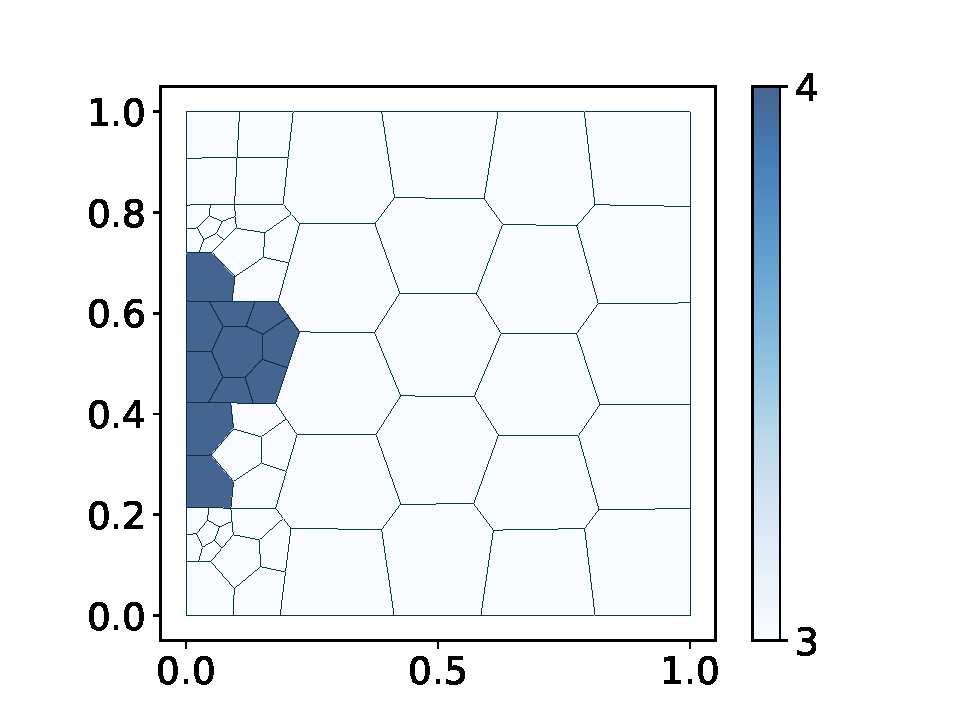
\includegraphics[width=5.5cm]{meshes/adaptive/square_hp_2.pdf}
	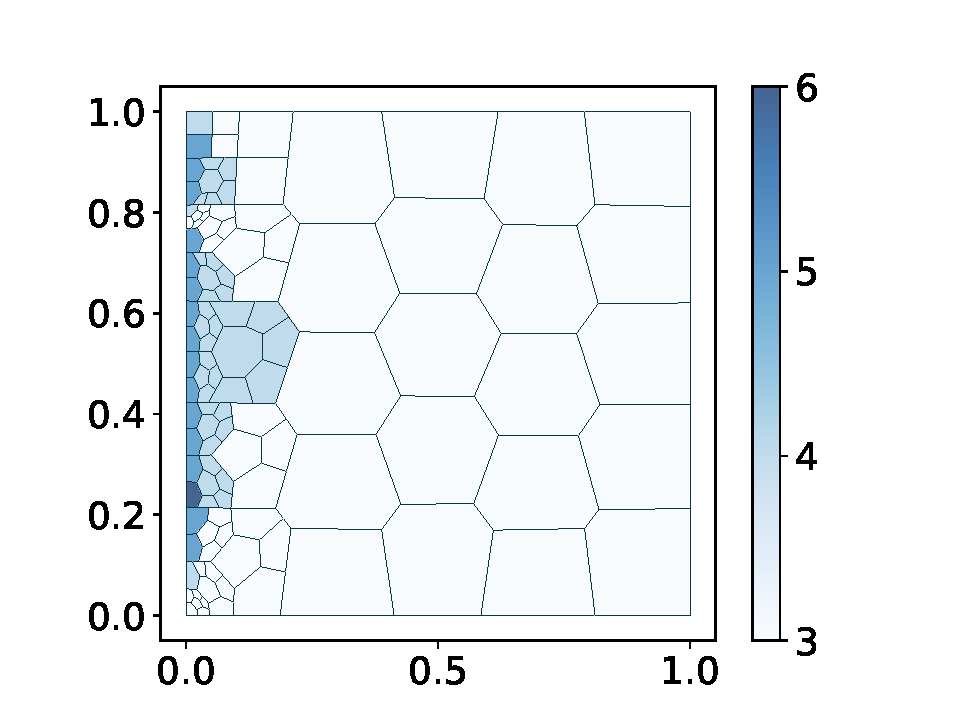
\includegraphics[width=5.5cm]{meshes/adaptive/square_hp_5.pdf}
	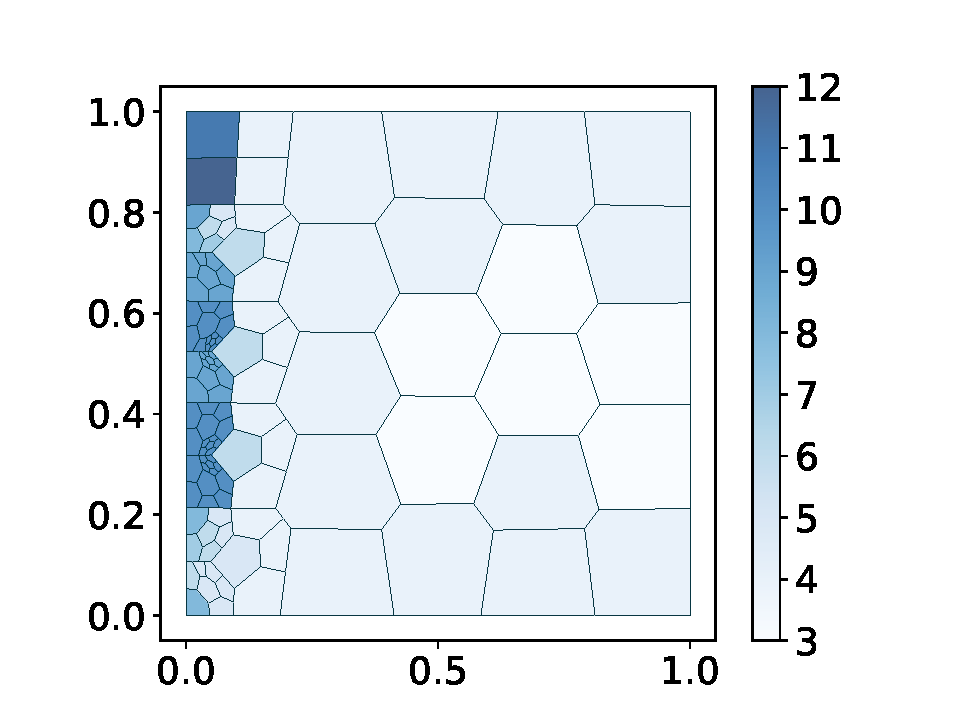
\includegraphics[width=5.5cm]{meshes/adaptive/square_hp_10.pdf}
    % 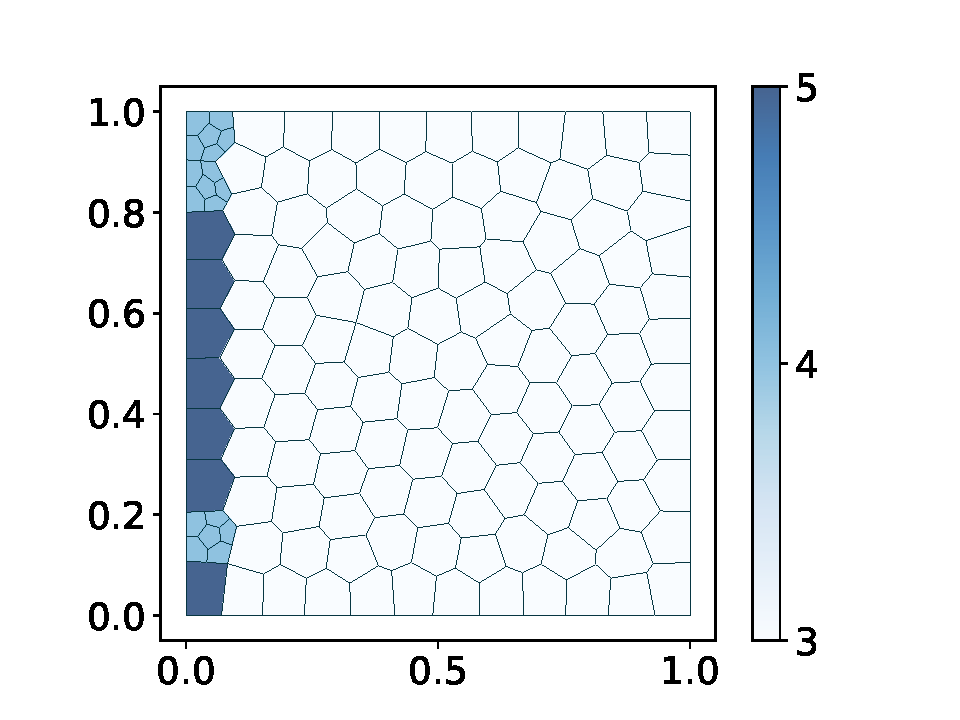
\includegraphics[width=5.5cm]{meshes/adaptive/square_hp_125_2.pdf}
	% 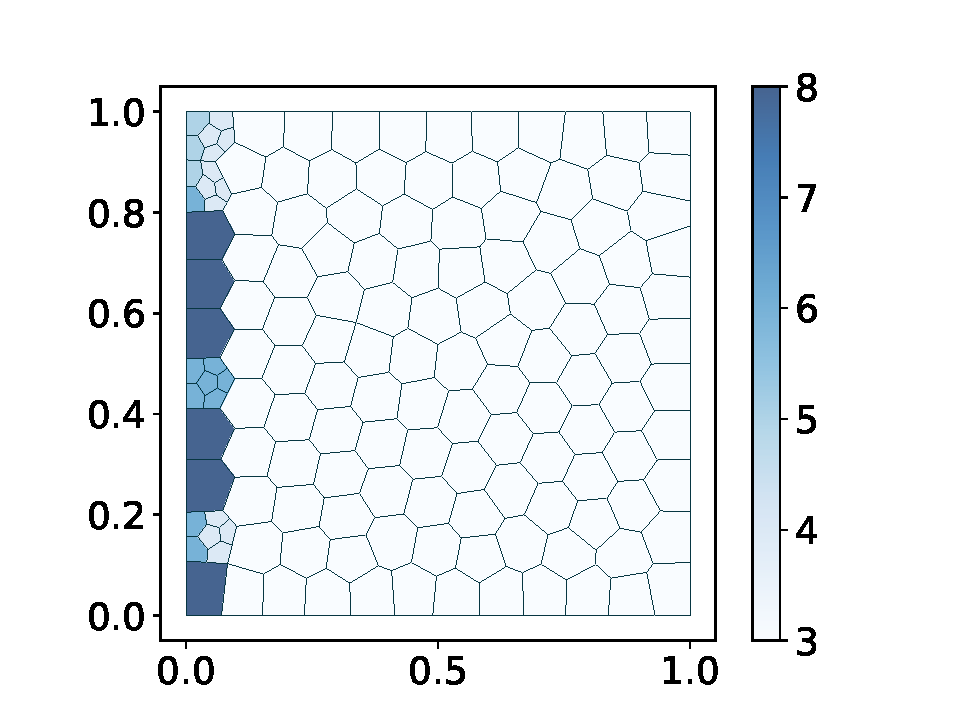
\includegraphics[width=5.5cm]{meshes/adaptive/square_hp_125_5.pdf}
	% 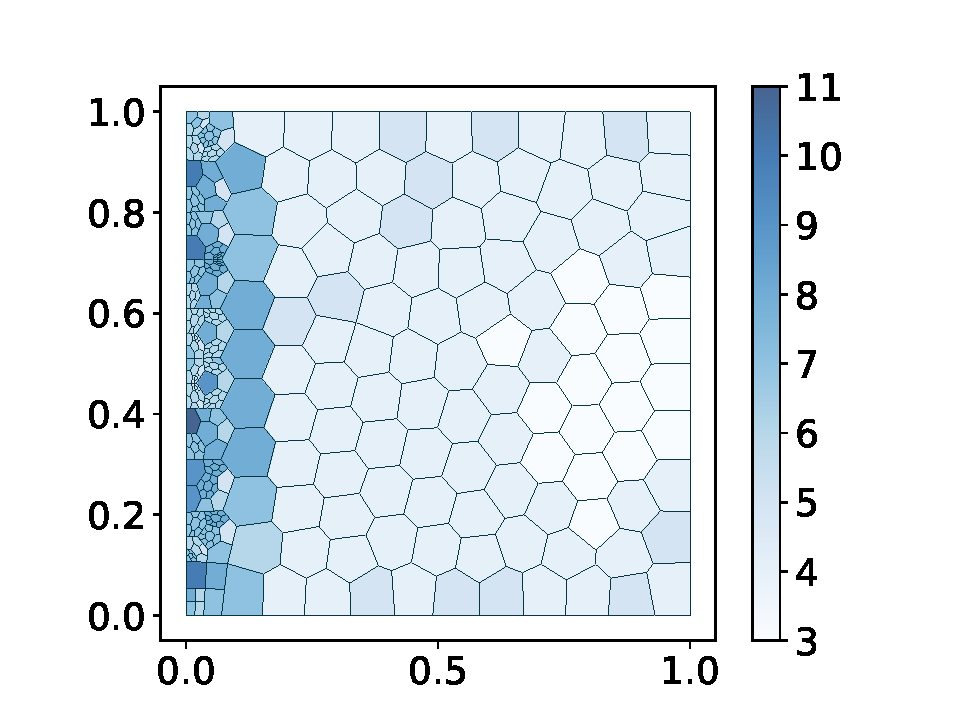
\includegraphics[width=5.5cm]{meshes/adaptive/square_hp_125_10.pdf}
	\caption{Square mesh after 2, 5 and 10 refinements, $N_0 = 25$ (top) and $N_0 = 125$ (bottom).}
\end{figure}

\begin{figure}[!ht]
	\centering
	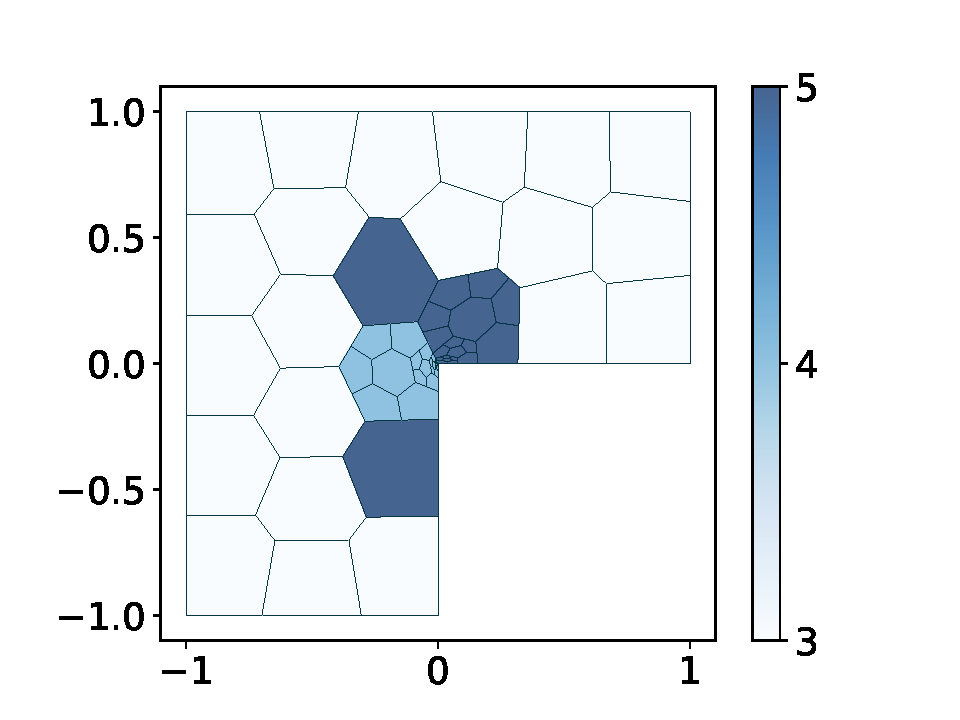
\includegraphics[width=5.5cm]{meshes/adaptive/lshape_hp_5.pdf}
	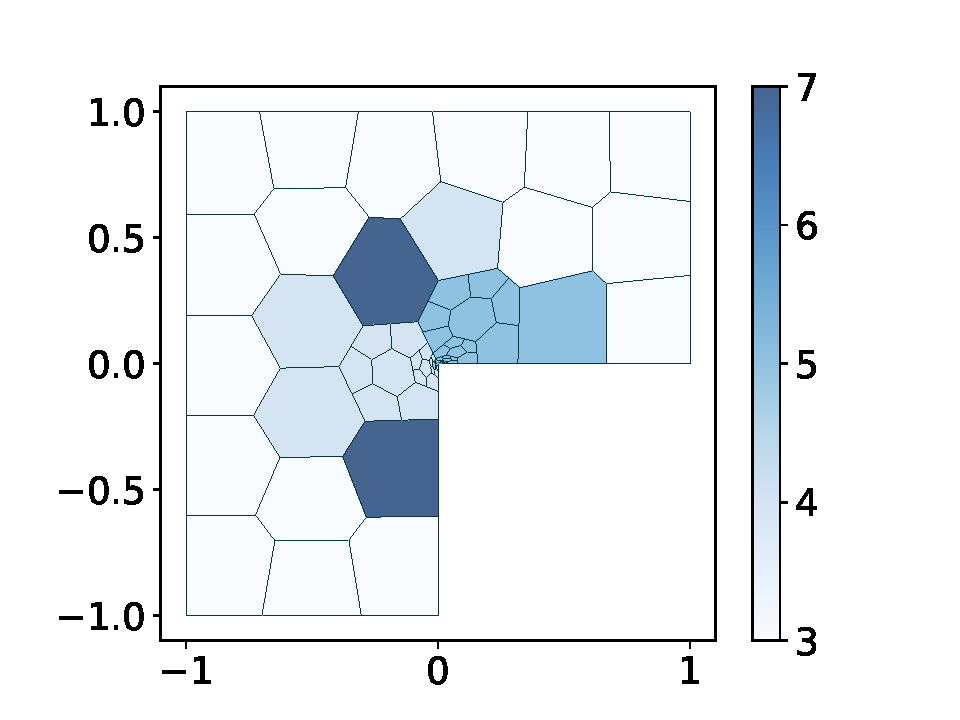
\includegraphics[width=5.5cm]{meshes/adaptive/lshape_hp_10.pdf}
	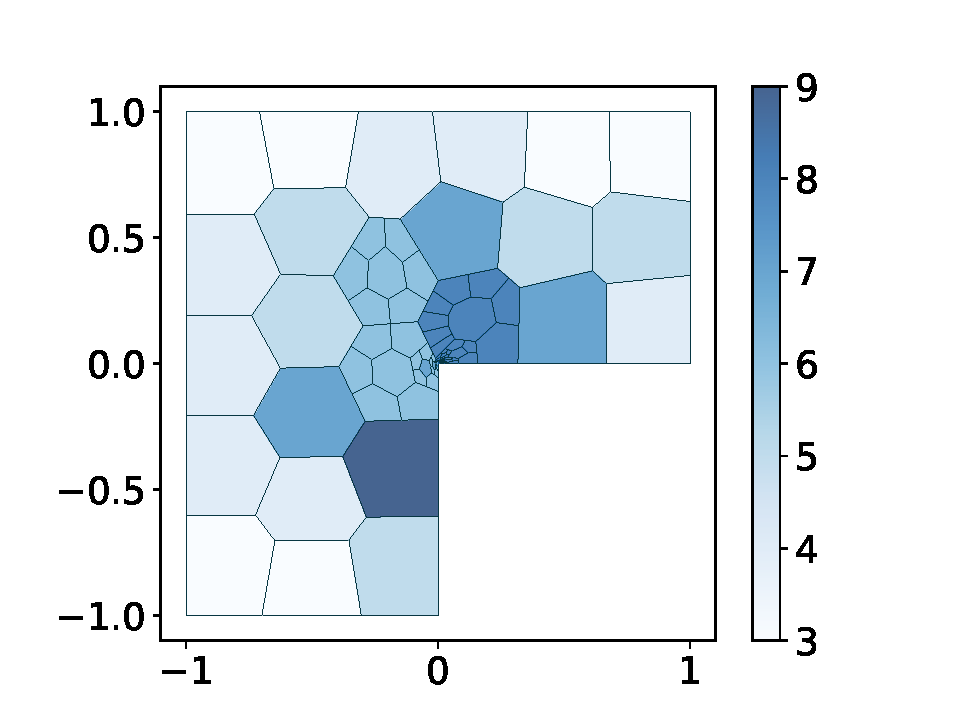
\includegraphics[width=5.5cm]{meshes/adaptive/lshape_hp_15.pdf}
    % 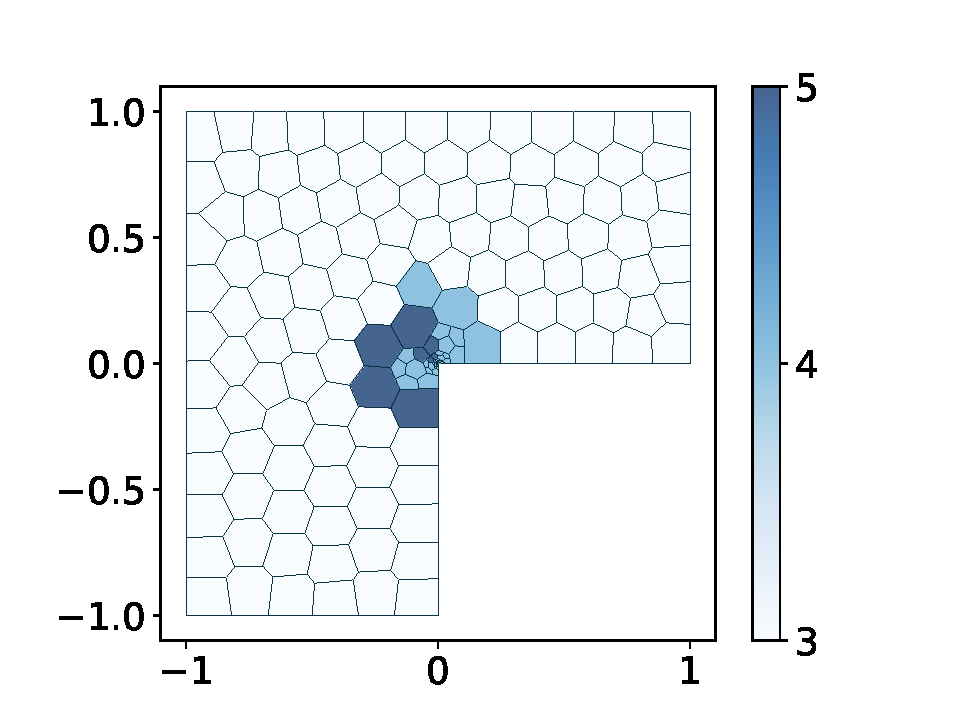
\includegraphics[width=5.5cm]{meshes/adaptive/lshape_hp_125_5.pdf}
	% 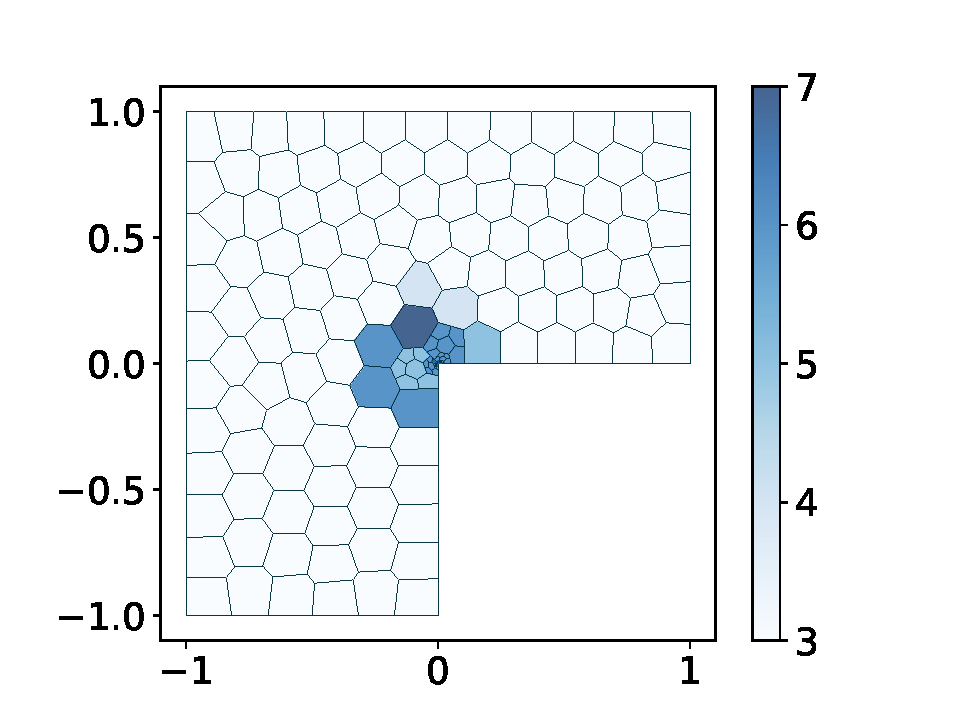
\includegraphics[width=5.5cm]{meshes/adaptive/lshape_hp_125_10.pdf}
	% 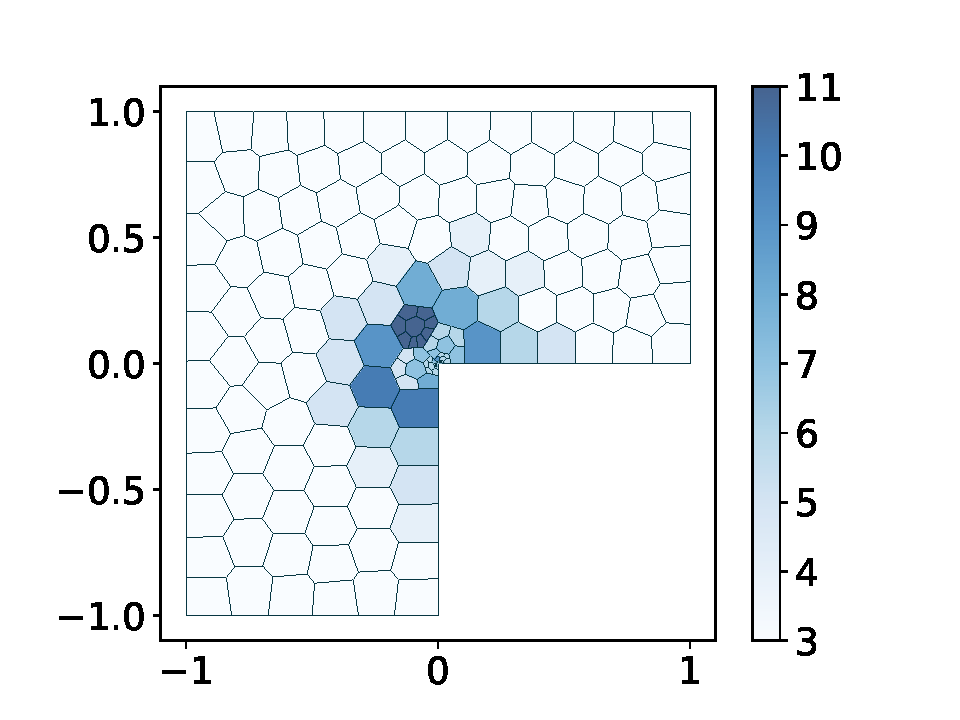
\includegraphics[width=5.5cm]{meshes/adaptive/lshape_hp_125_15.pdf}
	\caption{L-shaped mesh after 5, 10 and 15 refinements, $N_0 = 25$ (top) and $N_0 = 125$ (bottom).}
\end{figure}

\newpage
\subsection{A code snippet}

Here's a snippet to illustrate the \textit{hp-adaptive} mesh refinement from the user's perspective:

\lstinputlisting[style=cpp, firstline=11]{../snippets/hp_refine.cpp}